% ============================================================
%  RÉSUMÉ & ABSTRACT
% ============================================================
\chapter*{Résumé}
\addcontentsline{toc}{chapter}{Résumé}
\thispagestyle{plain}

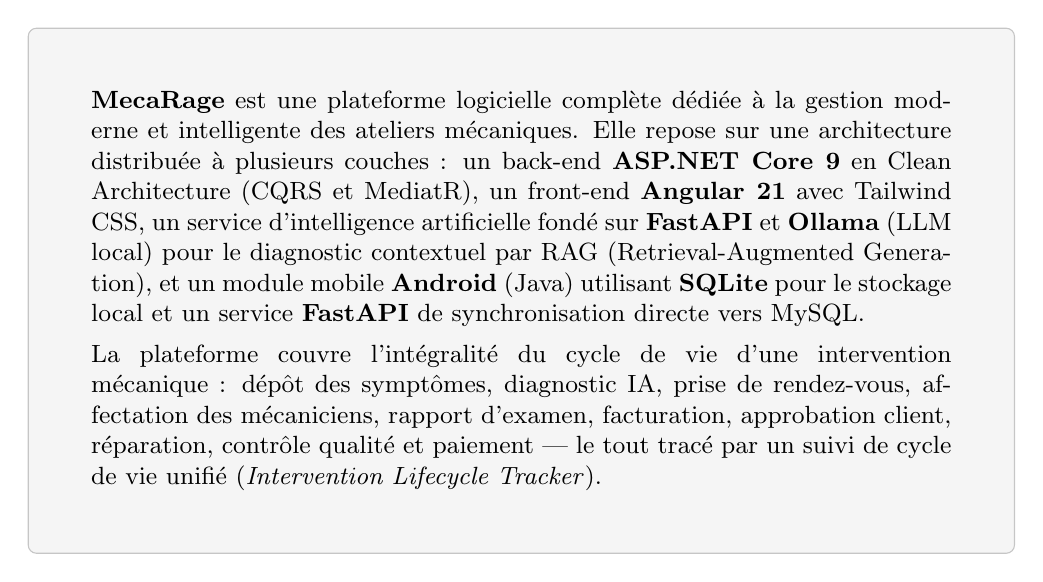
\begin{tikzpicture}
  \node[rectangle,fill=gray!8,draw=gray!45,rounded corners=3pt,
        text width=\dimexpr\linewidth-1.2cm\relax,inner sep=0.8cm,
        align=justify,font=\small] {
    \textbf{MecaRage} est une plateforme logicielle complète dédiée à la
    gestion moderne et intelligente des ateliers mécaniques. Elle repose sur
    une architecture distribuée à plusieurs couches~: un back-end
    \textbf{ASP.NET Core 9} en Clean Architecture (CQRS et MediatR), un
    front-end \textbf{Angular 21} avec Tailwind CSS, un service
    d'intelligence artificielle fondé sur \textbf{FastAPI} et
    \textbf{Ollama} (LLM local) pour le diagnostic contextuel par RAG
    (Retrieval-Augmented Generation), et un module mobile \textbf{Android}
    (Java) utilisant \textbf{SQLite} pour le stockage local et un service \textbf{FastAPI} de synchronisation directe vers MySQL.\\[0.4em]
    La plateforme couvre l'intégralité du cycle de vie d'une intervention
    mécanique~: dépôt des symptômes, diagnostic IA, prise de rendez-vous,
    affectation des mécaniciens, rapport d'examen, facturation, approbation
    client, réparation, contrôle qualité et paiement --- le tout tracé par un
    suivi de cycle de vie unifié (\textit{Intervention Lifecycle Tracker}).
  };
\end{tikzpicture}

\bigskip
\noindent\textbf{Mots-clés~:} Gestion d'atelier, Clean Architecture, CQRS,
Angular 21, ASP.NET Core 9, SQLite, FastAPI, Intelligence Artificielle, RAG, Android, MySQL.

\cleardoublepage

% ——————————————————————————————————————————————————————————
\chapter*{Abstract}
\addcontentsline{toc}{chapter}{Abstract}
\thispagestyle{plain}

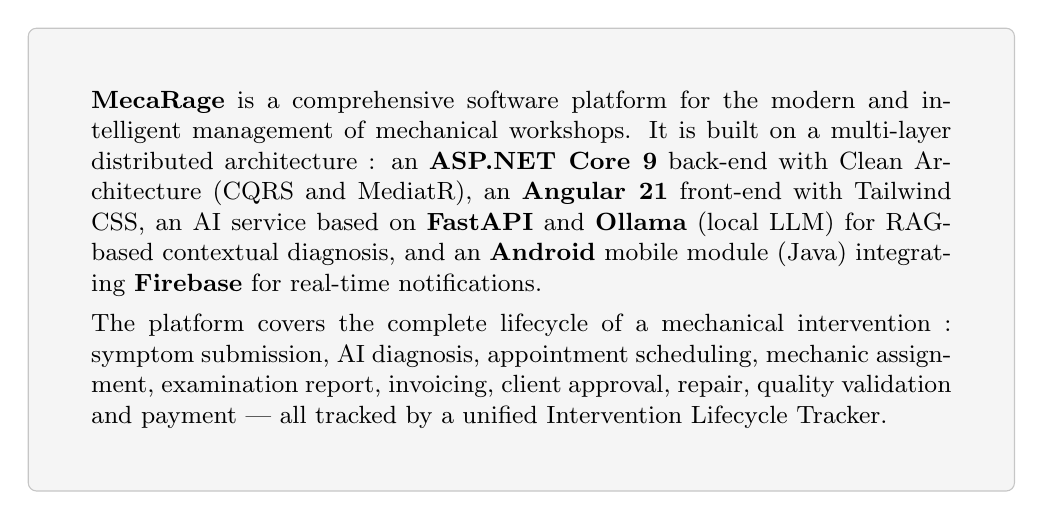
\begin{tikzpicture}
  \node[rectangle,fill=gray!8,draw=gray!45,rounded corners=3pt,
        text width=\dimexpr\linewidth-1.2cm\relax,inner sep=0.8cm,
        align=justify,font=\small] {
    \textbf{MecaRage} is a comprehensive software platform for the modern
    and intelligent management of mechanical workshops. It is built on a
    multi-layer distributed architecture~: an \textbf{ASP.NET Core 9}
    back-end with Clean Architecture (CQRS and MediatR), an
    \textbf{Angular 21} front-end with Tailwind CSS, an AI service based on
    \textbf{FastAPI} and \textbf{Ollama} (local LLM) for RAG-based contextual
    diagnosis, and an \textbf{Android} mobile module (Java) integrating
    \textbf{Firebase} for real-time notifications.\\[0.4em]
    The platform covers the complete lifecycle of a mechanical intervention~:
    symptom submission, AI diagnosis, appointment scheduling, mechanic
    assignment, examination report, invoicing, client approval, repair,
    quality validation and payment~--- all tracked by a unified Intervention
    Lifecycle Tracker.
  };
\end{tikzpicture}

\bigskip
\noindent\textbf{Keywords~:} Workshop management, Clean Architecture, CQRS,
Angular 21, ASP.NET Core 9, SQLite, FastAPI, Artificial Intelligence, RAG, Android, MySQL.

\cleardoublepage
